\documentclass[border=8pt]{standalone}
\usepackage[utf8]{inputenc}
\usepackage{tikz}
\usetikzlibrary{positioning}

\tikzset{
  entita/.style = {rectangle, draw, thick, fill=blue!8, minimum width=34mm, minimum height=14mm, font=\small},
  attr/.style   = {circle, draw, thick, fill=white, minimum size=5pt, inner sep=0},
  pk/.style     = {circle, draw, thick, fill=black, minimum size=5pt, inner sep=0},
  link/.style   = {thick},
  et/.style     = {font=\footnotesize}
}

\begin{document}
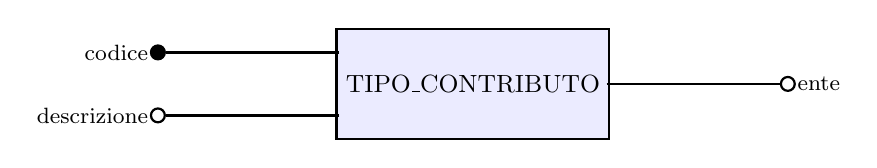
\begin{tikzpicture}
  \node[entita] (E) {TIPO\_CONTRIBUTO};
  \node[pk]   (c) at (-4.0, 0.4){}; \draw[link] (-1.7, 0.4)--(c); \node[et,left] at (c) {codice};
  \node[attr] (d) at (-4.0,-0.4){}; \draw[link] (-1.7,-0.4)--(d); \node[et,left] at (d) {descrizione};
  \node[attr] (e) at ( 4.0, 0.0){}; \draw[link] ( 1.7, 0.0)--(e); \node[et,right] at (e) {ente};
\end{tikzpicture}
\end{document}
